\section{Dinámicas factorizables}

En la sección \ref{sec:Ch1PartialTrace} se habló de estados separables como aquellos estados que, descritos por un operador de densidad $\rho\in\densityspace{n}$, tienen la forma
\begin{equation}
    \rho=\rho_{A}\otimes\rho_{B},\nonumber
\end{equation}
donde $\rho_{A}\in\densityspace{m}$, $\rho_{B}\in\densityspace{l}$ y $l+m=n$. Siguiendo esta línea de pensamiento, con \textit{dinámicas factorizables} nos referimos a dinámicas unitarias generadas por hamiltonianos que no contienen un término de interacción (que en el caso de dos partículas son hamiltonianos de la forma $\mcH=H_{1}\otimes\Id+\Id\otimes H_{2}$), y que por lo mismo son descritas por operadores $\mcU\in\unitaryspace{n}$ del tipo
\begin{equation}
    \mcU=U_{A}\otimes U_{B}.\nonumber
\end{equation}
De nuevo, $U_{A}\in\unitaryspace{m}$, $U_{B}\in\unitaryspace{l}$ y $l+m=n$. Los operadores separables están compuestos por operadores que actúan de forma independiente sobre diferentes subsistemas del sistema en cuestión. En el caso de un sistema compuesto por dos subsistemas de dos niveles, el operador separable está compuesto por dos unitarias que actúan sobre $\hilbert_{2}$. Como el estado de máxima entropía resulta ser separable, las dinámicas separables son una muy buena primera forma de aplicar el formalismo descrito en las secciones anteriores.

Considérese la aplicación de grano grueso de $n$ a $1$ partículas definida según (\ref{eq:CG}), un estado efectivo $\rho_{\ef}\in\densityspace{2}$ y la aplicación de máxima entropía compatible dada por (\ref{eq:MaxEntAss}). Si la evolución microscópica es factorizable entonces es generada por un hamiltoniano de la forma
\begin{equation*}
    \mcH=\sum_{k=1}^{n}\omega_{k}\Id_{2^{k-1}}\otimes H_{k} \otimes \Id_{2^{n-k}},
\end{equation*}
siendo la unitaria 
\begin{equation}\label{eq:NFactorUnitaries}
    \mcU_{t}=\Motimes_{k=1}^{n}\text{exp}\qty(-\rmi\omega_{k}H_{k}t)=\Motimes_{k=1}^{n} U_{k}(t).
\end{equation}
A partir de este momento, para hacer más limpia la lectura de este documento se omitirán los productos tensoriales con operadores identidad. El subsistema sobre el que actúe un operador será denotado por un subíndice, de tal manera que el hamiltoniano previamente definido queda
\begin{equation*}
    \mcH=\sum_{k=1}^{n}\omega_{k}H_{k}.
\end{equation*}


\subsection{Caso general}

Si se considera una evolución unitaria de la forma (\ref{eq:NFactorUnitaries}), y se propaga al estado obtenido de la aplicación de máxima entropía, el estado evolucionado es
\begin{equation}
    \varrho_{\max}(t)=\Motimes_{k=1}^{n}\frac{1}{Z_{k}}U_{k}(t) e^{\qty(p_{k}\sum_{j}\lambda_{j}\pauli{j})} (U_{k}(t))^{\dag}\nonumber
\end{equation}
El estado efectivo evolucionado en términos de los multiplicadores de Lagrange queda
\begin{equation}\label{eq:SeparableEvolution}
    \Gamma_{t}(\rho_{\ef})=\sum_{k=1}^{n}p_{k} U_{k}(t) \rho_{k} (U_{k}(t))^{\dag}.
\end{equation}
donde $\rho_{k}=\frac{1}{Z_{k}}e^{\qty(p_{k}\sum_{j}\lambda_{j}\pauli{j})}$. 

Por supuesto, esta expresión puede expandirse en términos de exponenciales o de funciones hiperbólicas del vector de Bloch del estado efectivo inicial, $\vec{r}_{\ef}$. Haciendo esto se obtiene una expresión para el valor esperado de $\pauli{j}$ a un tiempo $t$,
\begin{equation}\label{eq:SeparableEvolutionExpVal}
    \expval{\pauli{i}(t)}=\frac{1}{2}\sum_{k=1}^{n}p_{k}\tanh(p_{k}\lambda)\Tr[\pauli{j}U_{k}(t) (\hat{r}_{\ef}\cdot\vec{\sigma}) (U_{k}(t))^{\dag}]
\end{equation}
Si se piensa en el caso en que $p_{1}>p_{j}\,\forall j\neq 1$, separar la contribución del sistema de interés,
\begin{align}
    \expval{\pauli{j}(t)}=&\frac{1}{2}p_{1}\tanh(p_{1}\lambda)\Tr[\pauli{j}U_{1}(t) (\hat{r}_{\ef}\cdot\vec{\sigma}) (U_{1}(t))^{\dag}]\nonumber\\
    &+\frac{1}{2}\sum_{k=2}^{n}p_{k}\tanh(p_{k}\lambda)\Tr[\pauli{j}U_{k}(t) (\hat{r}_{\ef}\cdot\vec{\sigma}) (U_{k}(t))^{\dag}]\nonumber,
\end{align}
permite reconocer dos términos: uno asociado a la evolución \textit{sin error} de nuestro sistema, descrita por el operador unitario $U_{1}(t)$, y un término de ruido. La acción de este término dependerá tanto de la naturaleza de las evoluciones locales del entorno, como del número de partículas en este.


Por otro lado, en el caso en el que no hay partícula prioritaria, \ie ($p_{j}=\frac{1}{n}\forall j$), la relación entre la magnitud del vector de Bloch del estado efectivo y los multiplicadores de Lagrange es $\lambda=n\tanh^{-1}(r)$. Esto significa que la expresión del valor esperado de $\sigma_{j}$ a un tiempo $t$ es
\begin{equation}
    \expval{\pauli{j}(t)}=\frac{1}{2n}\sum_{k=1}^{n}\Tr[\pauli{j}U_{k}(t) (\vec{r}_{\ef}\cdot\vec{\sigma}) (U_{k}(t))^{\dag}],\nonumber
\end{equation}
que no es más que una combinación lineal de las mismas componentes evolucionadas de formas diferentes.
\subsection{Ejemplos particulares}

\subsubsection{Dinámica simétrica}

Comenzamos con el caso en el que la dinámica separable simétrica, esto es, de una unitaria $\mcU\in\unitaryspace{2^{n}}$ de la forma
\begin{equation}
    \mcU_{t}=\Motimes_{k=1}^{n}U(t),\nonumber
\end{equation}
donde $U(t)\in\unitaryspace{2}$. Se aplica la evolución al estado de máxima entropía compatible con un conjunto de observables tomográficamente completos en $\hilbert_{2}$ y se propaga al estado con la unitaria subyacente, para luego pasarlo por la aplicación de grano grueso y recuperar el estado efectivo evolucionado. Este caso es quizá el más sencillo, pues la simetría de la unitaria permite factorizarla:
\begin{align}
\mcC\qty[\Motimes_{k=1}^{n}U(t) \rho_{k} (U(t))^{\dag}]&=\sum_{k=1}^{n}p_{k} U(t) \rho_{k} (U(t))^{\dag}\nonumber \\
&=U(t)\qty(\sum_{k=1}^{n}p_{k} \rho_{k}) (U(t))^{\dag}\nonumber\\
&=U(t)\rho_{\ef}(U(t))^{\dag}.\nonumber
\end{align}
La dinámica efectiva tiene la forma
\begin{equation}
    \Gamma_{t}(\rho_{\ef})=U(t)\rho_{\ef}(U(t))^{\dag}.\nonumber
\end{equation}
Este resultado es natural. No solo no hay interacción entre los diferentes subsistemas, significando esto que no se \textit{filtra} ningún tipo de información entre la partícula de interés y el resto, sino que cada parte evoluciona de manera idéntica: bajo la aplicación de grano grueso, lo que se observa es una combinación de $n$ entidades idénticas evolucionando de la misma forma.

\subsubsection{Particulas no preferenciales invariantes}

Centrémonos, momentáneamente, en el régimen $p_{1}>p_{j}\,\forall j\neq 1$. Asúmase que la probabilidad de detectar a la $k$-ésima partícula es la misma para todas excepto la primera. Entonces
\begin{equation}
    p_{k}=\frac{(1-p_{1})}{n-1}\text{ }\forall k\neq 1.\nonumber
\end{equation}
El estado de máxima entropía compatible con un estado efectivo $\rho_{\ef}$ es
\begin{equation}
    \varrho_{\max}=\rho_{1}\otimes\qty(\Motimes_{k=2}^{n}\frac{1}{Z_{k}}e^{\frac{(1-p_{1})}{n-1}\sum_{j}\lambda_{j}\pauli{j}}),\nonumber
\end{equation}
donde, para todo $k$ se cumple que
\begin{equation}
    \frac{1}{Z_{k}}e^{\frac{1-p_{1}}{n-1}\sum_{j}\lambda_{j}\pauli{j}}=\frac{1}{2}\qty(\Id+\tanh(\frac{1-p_{1}}{n-1}\lambda)\hat{r}_{\rho}\cdot\vec{\sigma})\equiv \rho_{2}.\nonumber
\end{equation}
El conjunto de partículas no preferenciales es entonces
\begin{equation}
    \Motimes_{k=2}^{n}\rho_{k}=\rho_{2}^{\otimes(n-1)}\nonumber.
\end{equation}
Si estas no varían, mientras que el subsistema de interés se propaga de forma unitaria, entonces la dinámica efectiva es
\begin{equation}
    \Gamma_{t}(\rho_{\ef})=p_{1}U(t)\rho_{1}(U(t))^{\dag}+(1-p_{1})\rho_{2}.\nonumber
\end{equation}
En términos del vector de Bloch del estado efectivo inicial, con $r_{1}=\tanh(p_{1}\lambda)$, $r_{2}=\tanh((1-p_{1})\lambda)$, y $R$ la rotación generada por $U$:
\begin{equation}
    r_{\ef}\hat{r}_{\ef}\mapsto p_{1}r_{1}R\hat{r}_{\ef}+(1-p_{1})r_{2}\hat{r}_{\ef}.\nonumber
\end{equation}
Esta expresión parece no dar demasiada información: es simplemente la combinación lineal de dos vectores de Bloch, uno que ha sido rotado y otro al que no se le ha hecho nada, pero recordando que el vector de Bloch del estado efectivo inicial cumple $r=p_{1}r_{1}+(1-p_{1})r_{2}$, esta puede ser manipulada para ver que
\begin{equation}
    r\hat{r}_{\rho}\mapsto R(r\hat{r}_{\rho}-(1-p_{1})r_{2}\hat{r}_{\rho})+(1-p_{1})r_{2}\hat{r}_{\rho}.\nonumber
\end{equation}
El resultado es una rotación alrededor de una línea que no pasa por el origen. Una rotación de esta naturaleza puede descomponerse en una rotación a través de un eje que pasa por el origen $R_{0}$ y una traslación $T$ como $T^{-1}\circ R_{0}\circ T$. Nótese que una transformación así no tendría por qué mantener a los estados dentro de la esfera de Bloch, por lo que esta debe depender del estado mismo. 

\begin{figure}[ht!]
    \centering
    \begin{subfigure}{0.32\textwidth}
      \centering
      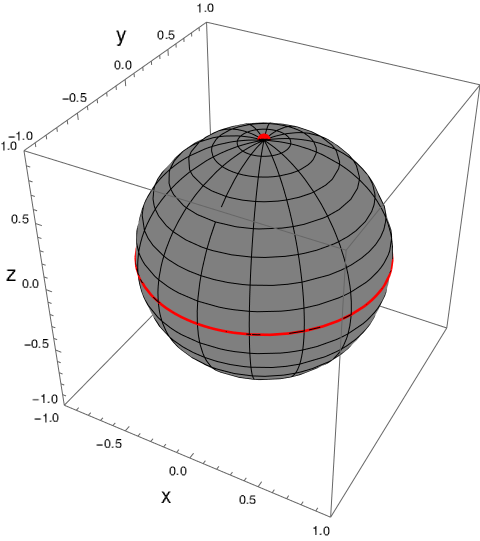
\includegraphics[width=0.9\linewidth]{chapter3/figures_separable/U1xU2_H1=Pi(sz)_H2=Id_z=0.9_p=0.6t=0.png}
      \caption{$t=0.0$}
    \end{subfigure}%
    \begin{subfigure}{0.32\textwidth}
      \centering
      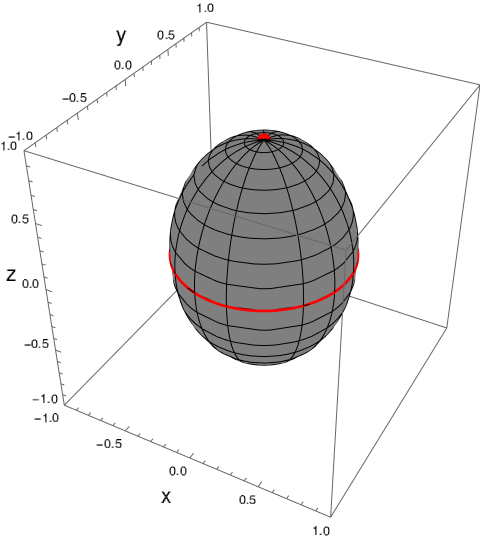
\includegraphics[width=0.9\linewidth]{chapter3/figures_separable/U1xU2_H1=Pi(sz)_H2=Id_z=0.9_p=0.6t=0.25.png}
      \caption{$t=0.25$}
    \end{subfigure}
    \begin{subfigure}{0.32\textwidth}
      \centering
      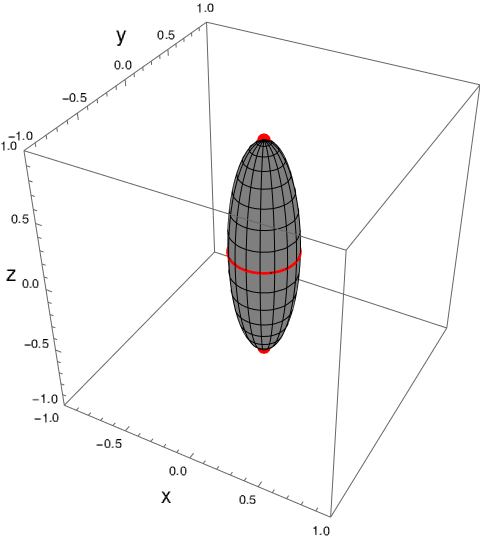
\includegraphics[width=0.9\linewidth]{chapter3/figures_separable/U1xU2_H1=Pi(sz)_H2=Id_z=0.9_p=0.6t=0.5.png}
      \caption{$t=0.5$}
    \end{subfigure}
    \caption{Efecto de la evolución subyacente sobre la esfera de Bloch si $r_{\ef}=0.9$, $p_{1}=0.6$ y $U=e^{-i\pi t \pauli{3}}$. La dramática contracción a lo largo de $z$ se asocia al alto valor de $1-p_{1}$.}
    \label{fig:FaseChangeSequence}
\end{figure}

En efecto, la traslación tiene una magnitud $(1-p_{1})r_{2}$ (a notar que la traslación es pequeña, y corresponde al término de ruido) en la dirección opuesta a la del estado (i.e. depende del estado tanto en magnitud como en dirección). Así que, aunque esto podría parecer una transformación afín, no lo es, pues depende enteramente del estado. Esto significa que la evolución efectiva no es lineal, y no tiene expresión en términos de operadores de Kraus. La figura \ref{fig:FaseChangeSequence} muestra el efecto que una dinámica de este estilo tiene sobre la esfera de Bloch (en particular, el caso $U_{1}=e^{-\rmi\omega t \pauli{3}}$). La contracción a lo largo del eje $z$ es un resultado del alto valor de $(1-p_{1})$ (0.4), y no sería visible si $p_{1}\rightarrow 1$.


En efecto, si $p_{1}\approx\frac{1}{2}$, entonces $\rho_{1}\approx\rho_{2}\approx\rho$ y la dinámica efectiva se convertiría en un canal de desfasamiento:

\begin{align}
    \Gamma_{t}(\rho_{\ef})=&p_{1}e^{-\rmi\omega t \pauli{3}}\rho_{1}e^{\rmi\omega t \pauli{3}}+(1-p_{1})\rho_{2}\nonumber\\
    \approx&\frac{1}{2}(\rho_{\ef}+e^{-\rmi\omega t \pauli{3}}\rho_{\ef} e^{\rmi\omega t \pauli{3}})\nonumber.
\end{align}

\subsubsection{Partícula preferencial invariante}

Ahora asumamos que es el sistema preferencial el que no evoluciona, mientras que las demás partículas sí lo hacen. Existen diferentes formas de abordar este problema, según la elección de las probabilidades y de la naturaleza de la evolución del entorno. Quizá el caso más sencillo es aquel en el que todas las partículas no preferenciales evolucionan de la misma forma. Esto es, una evolución generada por un hamiltoniano de la forma
\begin{equation}
    \mcH=\omega \sum_{k=2}^{n}H_{k}.\nonumber
\end{equation}
Por simplicidad, tómese $H_{k}=\pauli{3}\,\forall k$. Recordando la ecuación (\ref{eq:rhoArhoB}), los valores de expectación de $\pauli{j}$ serán
\begin{align}
    \expval{\pauli{1}(t)}=&p_{1} \expval{\sigma_{1}(0)}_{1}+\sum_{k=2}^{n}p_{k}\Tr[\pauli{1}e^{-\rmi\omega t\pauli{3}} \rho_{k} e^{\rmi\omega t\pauli{3}}]\nonumber\\
    \expval{\pauli{2}(t)}=&p_{1} \expval{\sigma_{2}(0)}_{1}+\sum_{k=2}^{n}p_{k}\Tr[\pauli{2}e^{-\rmi\omega t\pauli{3}} \rho_{k} e^{\rmi\omega t\pauli{3}}]\nonumber\\
    \expval{\pauli{3}(t)}=&\expval{\pauli{3}(0)}_{\ef},\nonumber
\end{align}
que quizá sea más clara escribiéndose en términos de las componentes de los vectores de Bloch de cada partícula (el primer subíndice indica la componente del vector, mientras que el segundo denota la partícula a la que pertenece):
\begin{align}
    r_{1}(t)=&r_{1,1}(0)+\sum_{k=2}^{n}p_{k}(r_{1,k}\cos(2\omega t)-r_{2,k}\sin(2\omega t))\nonumber\\
    r_{2}(t)=&r_{2,1}(0)+\sum_{k=2}^{n}p_{k}(r_{2,k}\cos(2\omega t)+r_{1,k}\sin(2\omega t))\nonumber\\
    r_{3}(t)=&r_{3,\ef}(0).\nonumber
\end{align}
Esto no es más que la aplicación de la misma rotación sobre todos los vectores de Bloch, a excepción del primero. Reescribiendo,
\begin{align}
    \vec{r}(t)=&p_{1}\vec{r}_{1}+R_{z}(2\omega t)\vec{r}_{e}\nonumber\\
    =&\vec{r}(0)+(R_{z}(2\omega t)-\Id)\vec{r}_{e}\nonumber
\end{align}
donde $\vec{r}_{e}\sum_{k=2}^{n}p_{k}\vec{r}_{k}$.
En este caso, el primer término es el término invariante, y sería lo único visible en el caso en que el aparato de medición no fallara, mientras que el segundo término corresponde a pequeñas oscilaciones completamente dependientes del estado efectivo inicial que nunca aumentan la pureza del estado. Estas pequeñas oscilaciones son, justamente, el término de ruido. La visualización a la solución del problema puede observarse en la Figura \ref{fig:OscilationsSameHam}. Cada una de las componentes del vector de Bloch efectivo se ve como una suma de una constante con funciones periódicas que tienen el mismo periodo, o  como la suma de una constante más una función periódica (viendo la combinación de los vectores de cada partícula del entorno como una partícula efectiva). De cualquier forma, el resultado es una función periódica.

\begin{figure}[ht!]
    \centering
    \begin{subfigure}{0.5\textwidth}
      \centering
      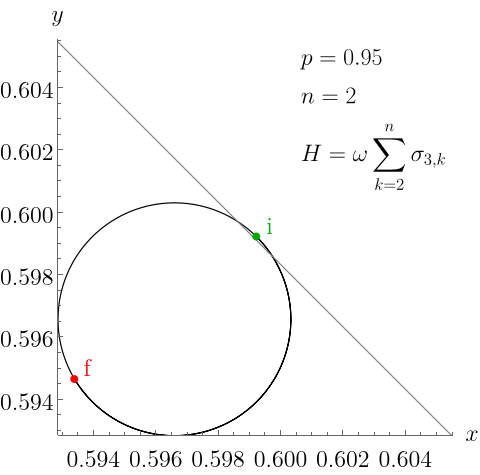
\includegraphics[width=0.9\linewidth]{chapter3/figures_separable/spheretraject_sameHam_difprob_n=2_p=0.95_both.png}
      \caption{Entorno de una partícula.}
    \end{subfigure}%
    \begin{subfigure}{0.5\textwidth}
      \centering
      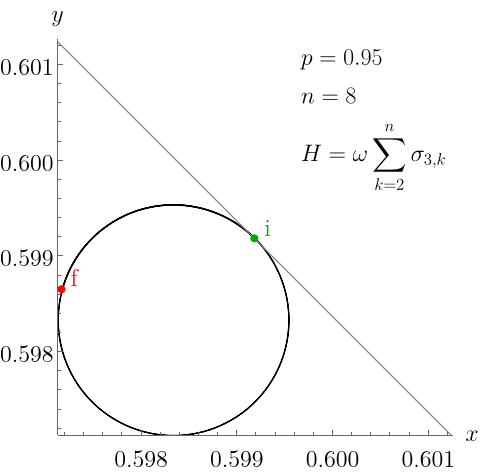
\includegraphics[width=0.9\linewidth]{chapter3/figures_separable/spheretraject_sameHam_difprob_n=8_p=0.95_both.png}
      \caption{Entorno de siete partículas.}
    \end{subfigure}
    \caption{Oscilaciones periódicas cercanas al valor esperado. La periodicidad no depende de los pesos probabilísticos de cada partícula. En gris, el conjunto de estados con la misma pureza (y la misma coordenada en $\pauli{3}$) que el estado efectivo inicial.}\label{fig:OscilationsSameHam}
\end{figure}

Si, por otro lado, quitamos la restricción de que todas las partículas del entorno evolucionen con la misma frecuencia, se vuelve imposible factorizar la rotación:
\begin{equation}
    \vec{r}(t)=p_{1}\vec{r}_{1}+\sum_{k=2}^{n} p_{k}R_{z}(2\omega_{k} t)\vec{r}_{k}.\nonumber
\end{equation}
Ahora cada partícula del entorno contribuye al error de forma única, y a pesar de que la evolución de cada partícula del entorno sea periódica, la combinación de estas no tiene por qué serlo. El resultado sigue siendo de oscilaciones cercanas a un valor \textit{sin error}. Las figuras \ref{fig:OscilationsNormalFreqSmallSigm} y \ref{fig:OscilationsNormalFreqBigSigm} muestran dichas oscilaciones para el caso en que las frecuencias se han obtenido a través de distribuciones normales de media $\mu=2$ y desviaciones estándar $\sigma=0.2$ y $\sigma=10$ respectivamente.

\begin{figure}[ht!]
    \centering
    \begin{subfigure}{0.5\textwidth}
      \centering
      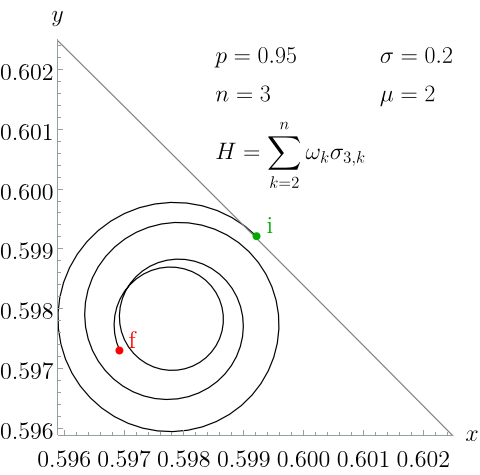
\includegraphics[width=0.9\linewidth]{chapter3/figures_separable/sphere_traject_sigmaz_normal_freq_mean=2_std=0.2_n=3_p=0.95_both.png}
      \caption{Dos partículas no preferenciales.}
    \end{subfigure}%
    \begin{subfigure}{0.5\textwidth}
      \centering
      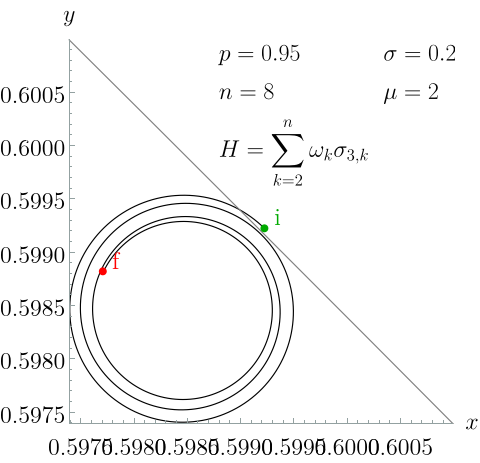
\includegraphics[width=0.9\linewidth]{chapter3/figures_separable/sphere_traject_sigmaz_normal_freq_mean=2_std=0.2_n=8_p=0.95_both.png}
      \caption{Siete partículas no preferenciales.}
    \end{subfigure}
    \caption{Oscilaciones periódicas cercanas al valor esperado. Las frecuencias de evolución fueron obtenidas de una distribución normal.}\label{fig:OscilationsNormalFreqSmallSigm}
\end{figure}

\begin{figure}[ht!]
    \centering
    \begin{subfigure}{0.5\textwidth}
      \centering
      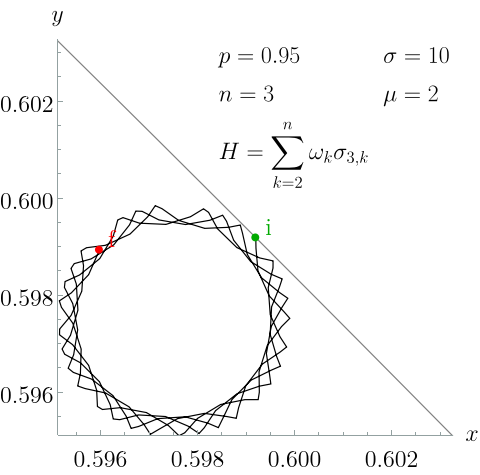
\includegraphics[width=0.9\linewidth]{chapter3/figures_separable/sphere_traject_sigmaz_normal_freq_mean=2_std=10_n=3_p=0.95_both.png}
      \caption{Dos partículas no preferenciales.}
    \end{subfigure}%
    \begin{subfigure}{0.5\textwidth}
      \centering
      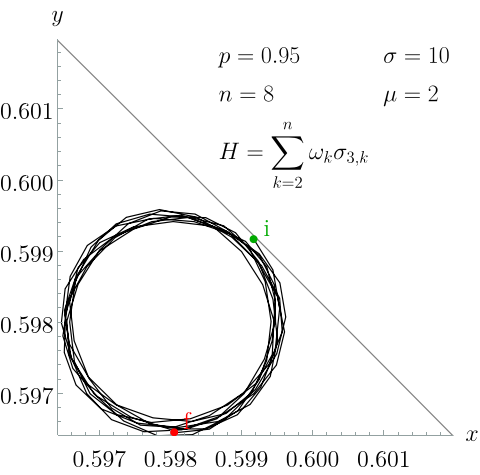
\includegraphics[width=0.9\linewidth]{chapter3/figures_separable/sphere_traject_sigmaz_normal_freq_mean=2_std=10_n=8_p=0.95_both.png}
      \caption{Siete partículas no preferenciales.}
    \end{subfigure}
    \caption{Oscilaciones periódicas cercanas al valor esperado. Las frecuencias de evolución fueron obtenidas de una distribución normal.}\label{fig:OscilationsNormalFreqBigSigm}
\end{figure}

\subsubsection{Sistema en campo magnético ?}

\acnote{No tengo idea de qué justificación se pueda dar a que todas las partículas oscilen en la misma dirección pero con frecuencias diferentes.}

En los dos casos anteriores se permitió que alguna de las partes del sistema se mantuviera invariante, fuera la partícula preferencial  o las partículas que conforman su entorno. Veamos ahora qué sucede cuando se permite que todo el sistema evolucione. Considérese un hamiltoniano
\begin{equation}
    \mcH=\sum_{k=1}^{n}\omega_{k}\Id_{2^{k-1}}\otimes \pauli{3} \otimes \Id_{2^{n-k}},\nonumber
\end{equation}
de tal forma que toda la evolución mantenga constante la componente en $\pauli{3}$. Además, como antes, obténganse las frecuencias de evolución de una distribución normal, con $\omega_{1}=\mu$.

\begin{figure}[ht!]
    \centering
    \begin{subfigure}{0.5\textwidth}
      \centering
      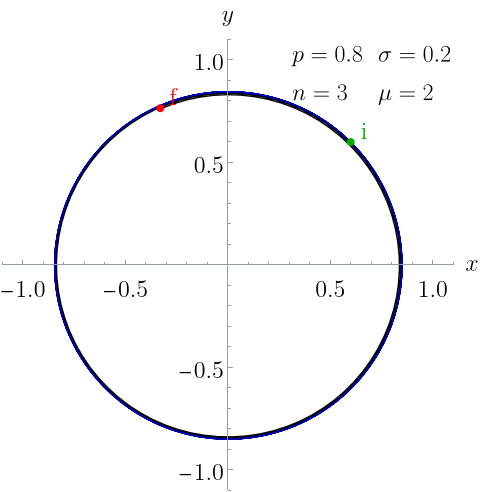
\includegraphics[width=0.9\linewidth]{chapter3/figures_separable/sphere_traject_ALL_sigmaz_normal_freq_mean=2_std=0.2_n=3_p=0.8_both.png}
    \end{subfigure}%
    \begin{subfigure}{0.5\textwidth}
      \centering
      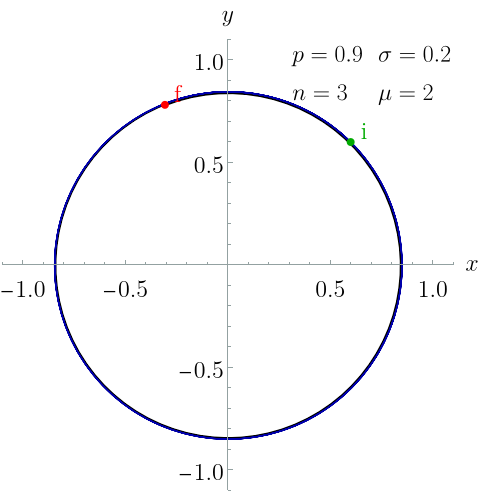
\includegraphics[width=0.9\linewidth]{chapter3/figures_separable/sphere_traject_ALL_sigmaz_normal_freq_mean=2_std=0.2_n=3_p=0.9_both.png}
    \end{subfigure}
    \caption{Oscilaciones periódicas cercanas al valor esperado. Como las frecuencias de las demás partículas son muy cercanas a la de la primera, casi no se observa error. Pero existe. \acnote{Tengo ploteado dicho error}}\label{fig:Oscilations12}
\end{figure}
\begin{figure}[ht!]
    \centering
    \begin{subfigure}{0.5\textwidth}
      \centering
      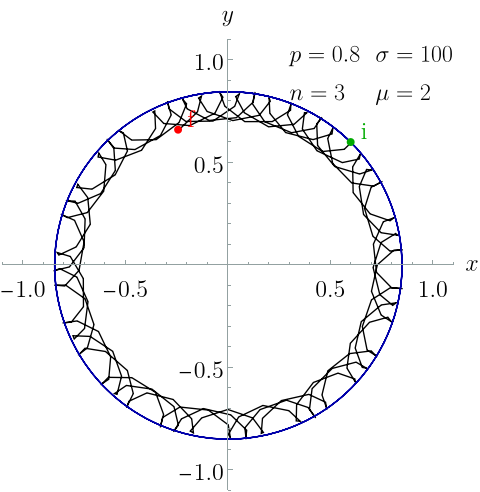
\includegraphics[width=0.9\linewidth]{chapter3/figures_separable/sphere_traject_ALL_sigmaz_normal_freq_mean=2_std=100_n=3_p=0.8_both.png}
    \end{subfigure}%
    \begin{subfigure}{0.5\textwidth}
      \centering
      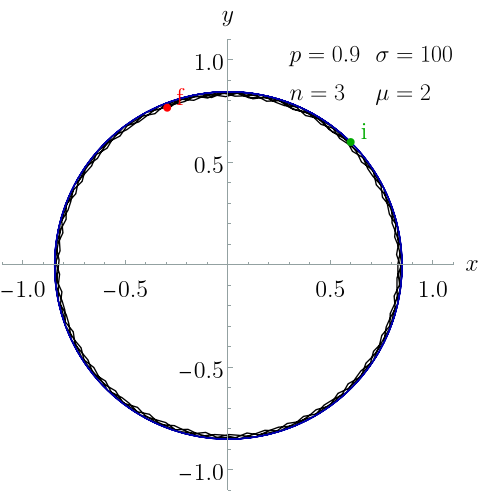
\includegraphics[width=0.9\linewidth]{chapter3/figures_separable/sphere_traject_ALL_sigmaz_normal_freq_mean=2_std=100_n=3_p=0.9_both.png}
    \end{subfigure}
    \caption{Trayectoria adecuada en azul. Las oscilaciones son más visibles conforme más pequeño es $p_{1}$ (o mayor el error). La alta desviación estándar permite ver las oscilaciones "bonitas"}\label{fig:Oscilations13}
\end{figure}

\newpage

\pagebreak